\section{Concrete implementation}
\label{sec:concrete}

The operational semantics we have derived in the previous section
constitutes an abstract \emph{specification}: a semantics for which
non-interference is (obviously) true.  This specification can guide the
design of an information-flow calculus which would not be directly
derivable from our procedure, but is related to some such derivation.
For example, in our mini-ML language, the combined semantics requires
each thread to have a separate ML heap.  In an actual implementation, we
might like to only have a single heap and disallow the passing of
references between threads.  This restriction maintains a correspondence
between the abstract multiple heaps and the concrete single heap.  We might
hope that we can prove noninterference for this new system by reusing
noninterference for the old system.

However, modifying operational rules poses a distinct problem for
preserving non-interference.  Consider a trivial state machine as shown
in Figure~\ref{fig:trivial-sm}, whose second projection is classified
secret.  With all three transitions, this language fulfills
termination-sensitive noninterference.  Furthermore, if the dashed line
is removed, the language continues to satisfy TSNI.  However, if any
solid line is removed, however, the language fails TSNI.

\begin{figure}
    States: $(x,y)$ for $x,y \in \{0,1\}$ \\
    Erasure function: $f(x,y) = (x,\bullet)$

    \begin{center}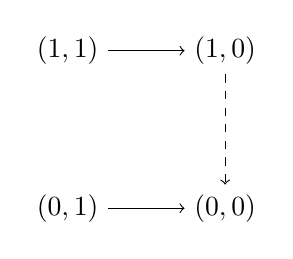
\begin{tikzpicture}[node distance=2cm, auto]
        \node (A) {$(1,1)$};
        \node (B) [right of=A] {$(1,0)$};
        \node (C) [below of=A] {$(0,1)$};
        \node (D) [right of=C] {$(0,0)$};
        \draw[->] (A) to node {} (B);
        \draw[->] (C) to node {} (D);
        \draw[->, dashed] (B) to node {} (D);
    \end{tikzpicture}\end{center}

    \label{fig:trivial-sm}
    \caption{A trivial state machine}
\end{figure}

The approach we will take is in two steps.  First, we sidestep the
restriction problem by demanding that the concrete implementation be
\emph{isomorphic} to the abstract specification, but perhaps having a different
runtime representation (a single heap) and some well-formedness
condition (every item on the heap only contains pointers from a single
location).  Isomorphism will preserve nonintereference, but it will also means all
transitions in the abstract language have to be implemented, including
undesirable transitions such as sending a pointer to another thread makes
the pointer dangling.  Next, we define a desugaring into this language
which adds dynamic checks, eliminating the possibility for these undesirable
transitions to be exercised.

\begin{theorem}[Isomorphism preserves termination sensitive non-interference]
    Consider a language \tar{L} with configurations |tc|, reduction
    relation \tar{|.->|} and erasure function \tar{|erasef l|} and a
    language \ifc{L} with configurations |ic|, reduction relation
    \ifc{|.->|} and erasure function \ifc{|erasef l|}.  We say that
    \tar{L} and \ifc{L} are isomorphic if there exist (total) functions
    $f : |tc -> ic|$ and $f^{-1} : |ic -> tc|$ such that $f \circ f^{-1}
    = id$, $f^{-1} \circ f = id$, and that $f$ and $f^{-1}$ are
    functorial over $l$-equivalences (i.e. if $|tc|\ \tar{\approx_l}\
    |tc'|$ then $f(|tc|)\ \ifc{\approx_l}\ f(|tc'|)$ and vice-versa).
    Then if \ifc{L} satisfies termination sensitive non-interference,
    then \tar{L} satisfies termination sensitive non-interference.
\end{theorem}

\begin{proof}
    Easily shown by transporting configurations and reduction derivations
    from \tar{L} to \ifc{L}, applying TSNI, and then transporting the resulting
    configuration and derivation back.
\end{proof}

\begin{figure}

\begin{mathpar}
\inferrule[I-stepT]
{|
conf tS (te) -> conf tS' te'
|}
{|
coconf iS tS (cconf id il (iniE (IT te)), ldots)
.->
iS ; tS' ; sched step (cconf id il (iniE (IT te')), ldots)
|}

\and
% This rule is not complete, needs the FV condition
\inferrule[C-fork]
{ 
|iS' = iS [ id' mapsto nil ]|\\
|it1 = cconf id il (iniE id')|\\
|itnew = cconf id' il (TI ie)|\\
|fresh (id')|
}
{|
coconf iS tS (lconf id il (iniE (fork ie)), ldots)
.->
iS'; tS; sched fork (it1, ldots, itnew)
|}
\end{mathpar}

\caption{ML with a single heap}
\label{fig:comb}
\end{figure}

This version
